\RHpresentationHead{
  \documentclass[pdftex,unicode,xcolor=table]{beamer}
}

\RHarticleHead{
  % This does not work, because of colors, \insertauthor, etc.
  \documentclass[a4paper,12pt,pdftex,unicode]{article}
  \usepackage[envcountsect]{beamerarticle}
}



\mode<presentation> {
  \usetheme{Fedora}
  \setbeamertemplate{navigation symbols}{}
  \setbeamercovered{transparent=5}
}
\mode<article> {
  \usepackage{fullpage}
}

\mode<handout> {
  \usepackage{pgfpages}
  \pgfpagesuselayout{4 on 1}[a4paper,landscape,border shrink=5mm]
}


\usepackage{beamerredhat}
\usepackage{etex}
\usepackage[utf8]{inputenc}
%\usepackage[lang]{babel}
\usepackage{setspace,amsfonts,calc,upquote,hyperref,floatflt,graphicx}
\usepackage[table]{xcolor}
\usepackage{colortbl}
\usepackage[absolute,overlay]{textpos}\textposquirk


% presentation title/author/etc.
\title{(R)evolution of Java packaging in GNU/Linux}
\subtitle{Automating packaging}
\author{Authors: \\
  \em{Stanislav Ochotnický} sochotnicky@redhat.com\\
  \em{Mikołaj Izdebski} mizdebsk@redhat.com}
\date{Date: \em{2nd February 2013}}


% fancy section/part pages?
% \fancySectionOpens
% \fancyPartOpens

\begin{document}


% title pages
\mode<article> {
  \maketitle
  \newpage
}

\begin{rhbg}
  \begin{frame}
    \titlepage
    \begin{abstract}
      Packaging Java in GNU/Linux distributions is complicated by incomplete
      tooling. Over past 2 years, tooling and guidelines for packaging Java have
      changed in Fedora considerably. What used to be a 1000 line build
      script can soon become 100 lines of mostly metadata.  We present new
      bleeding edge distribution-neutral tooling for packaging Maven artifacts.
    \end{abstract}
    \note{
    Just our introduction. We have been working in Java/Maven packaging for
    Fedora and Red Hat Enterprise Linux for several years. We like to make
    things simple(r).
    }
  \end{frame}
\end{rhbg}


\section{Overview}
\Large
\begin{frame}
  \frametitle{Why is there a problem in the first place?}
  \begin{itemize}
  \item Sort of NIH syndrome everywhere
  \item Each Java package a unique set of problems
    \begin{itemize}
      \item Ant, Maven, Gradle, Ivy, 20 XML parser dependencies
    \end{itemize}
  \item Each Linux distribution a unique set of problems
    \begin{itemize}
      \item RPM, APT, Portage, FHS, exceptions to FHS
    \end{itemize}
  \item Can we do better?
    \begin{itemize}
      \item Conventions
      \item Tooling
      \item Sharing
      \item Caring
    \end{itemize}
  \end{itemize}
  \note{NIH - distributions, java developers, everyone is guilty. If we manage
  to provide a proper tooling a lot of things will get better as a result eventually.}
\end{frame}

\begin{frame}
  \frametitle{First things first}
Maven is the only widely-used Java build tool with any resemblance of
      conventions

\begin{center}
\setlength{\tabcolsep}{2pt}
\small
\begin{tabular}{| c || c |} \hline
RPM & Maven \\ \hline
Name & \textless artifactId/\textgreater \\
Version & \textless version/\textgreater \\
(Build)Requires &  \textless dependencies/\textgreater \\
License & \textless licenses/\textgreater \\
\%summary & \textless name/\textgreater \\
\%description & \textless description/\textgreater \\
\%prep & \textless build/\textgreater \\
\%build & \textless build/\textgreater \\
\%install & \textless build/\textgreater \\
... & ... \\
\hline
\end{tabular}
\end{center}
  \note{Most things are very similar. But there are exceptions:
    \begin{itemize}
    \item Not all metadata is 1:1
    \item No exclusions in RPMs
    \item No equivalent of Maven scope in RPMs
    \item Parent pom inheritance missing
    \item Optional dependencies
    \end{itemize}

    The problem with other build systems is that there is no way to standardize
  parsing and handling of their metadata. They can be spread in many places.
  }
\end{frame}

\section{History lessons}
\begin{frame}
\frametitle{Maven modifications in Fedora}
\begin{itemize}
\item Custom resolver used in local mode
\item Verification of models turned off in local mode
\item Fix test scope dependency resolving when tests are disabled
\item Approximate idea is:
  \begin{itemize}
  \item Create a file that will map GAV to jars on filesystem
  \item Maven loads this file when running in local mode
  \item Return artifacts based on this mapping
  \end{itemize}
\end{itemize}
\note{Maven and Java stack largely based on JPP. It is our heritage, but we are
  changing it bit by bit. Our patches are not very welcome by the upstream, but
  we are getting rid of them.}
\end{frame}

\begin{frame}[fragile]
  \frametitle{Getting rid of cruft}
  \scriptsize
  \begin{block}{We had this in our spec files}
  \begin{verbatim}
Requires(post): jpackage-utils
Requires(postun): jpackage-utils

%post
%update_maven_depmap

%postun
%update_maven_depmap
\end{verbatim}
\end{block}
\begin{block}{Now we have}
\end{block}
\note{These snippets used to produce one big mapping file out of small xml-like
  files created by every Maven package. Maven then read this one big file. We
  moved to reading those small files and with this we didn't have to create the
  big file any more. Performance hit is negligible.}
\end{frame}



\begin{frame}[fragile]
\scriptsize
  \frametitle{Fixing manual mapping for GAVs}
  \begin{block}{Mapping between GAV and jar was manual}
\begin{verbatim}
%add_to_maven_depmap org.apache.commons commons-io 2.5 JPP commons-io
\end{verbatim}
  \end{block}
  \begin{block}{Better way with the same result}
\begin{verbatim}
%add_maven_depmap JPP-commons-io.pom commons-io.jar
\end{verbatim}
  \end{block}
  \note{This has been achieved by reading metadata from pom.xml instead of
  relying on manual inspection. We managed to get rid of a lot of errors this way}
\end{frame}


\begin{frame}[fragile]
  \scriptsize
\frametitle{Modifications of pom.xml}
  \begin{block}{Old style patching}
\begin{verbatim}
--- ./surefire-providers/pom.xml.sav
+++ ./surefire-providers/pom.xml
@@ -30,8 +30,10 @@
   <name>SureFire Providers</name>
   <modules>
     <module>surefire-junit</module>
+<!--
     <module>surefire-junit4</module>
     <module>surefire-testng</module>
+-->
   </modules>
   <dependencies>
     <dependency>
\end{verbatim}
\end{block}

  \begin{block}{New macros}
\begin{verbatim}
%pom_disable_module surefire-junit4
%pom_disable_module surefire-testng
\end{verbatim}
\note{There are other macros:
    \begin{itemize}
    \item adding/removing dependencies
    \item modifying plugins
    \item injecting/removing any xml parts
    \end{itemize}
    All in all they simplify updates and are more reliable than patches since
    they know about XML structure
}
\end{block}
\end{frame}


\begin{frame}[fragile]
  \scriptsize
\frametitle{File lists}
  \begin{block}{Manual listing}
\begin{verbatim}
%files
%defattr(-,root,root,-)
%doc LICENSE.txt NOTICE.txt RELEASE-NOTES.txt
%{_javadir}/*.jar
%{_mavenpomdir}/JPP-%{short_name}.pom
%{_mavendepmapfragdir}/*
\end{verbatim}
\end{block}

  \begin{block}{Automated way}
\begin{verbatim}
%files -f .mfiles
%doc LICENSE.txt NOTICE.txt RELEASE-NOTES.txt
\end{verbatim}
\note{These file lists are relatively limited in that they only handle files
that \%add\_maven\_depmap macro knows about: poms, jars, mapping files. They
still simplify spec files considerably
}
\end{block}
\end{frame}

\begin{frame}
  \frametitle{Current state}
  \begin{itemize}
    \item Simple issues were solved
    \item Most time-consuming tasks are still manual
    \begin{itemize}
      \item keeping dependencies up-to-date
      \item installing multi-artifact packages
      \item maintenance of multiple subpackages
    \end{itemize}
  \end{itemize}
  \note{Maintenance of multiple subpackages is always a burden. Dependencies get
  more complicated, spec files are much longer and their updates more error-prone.}
\end{frame}


\begin{frame}[fragile]
  \frametitle{Plexus-compiler example}
  \begin{center}
    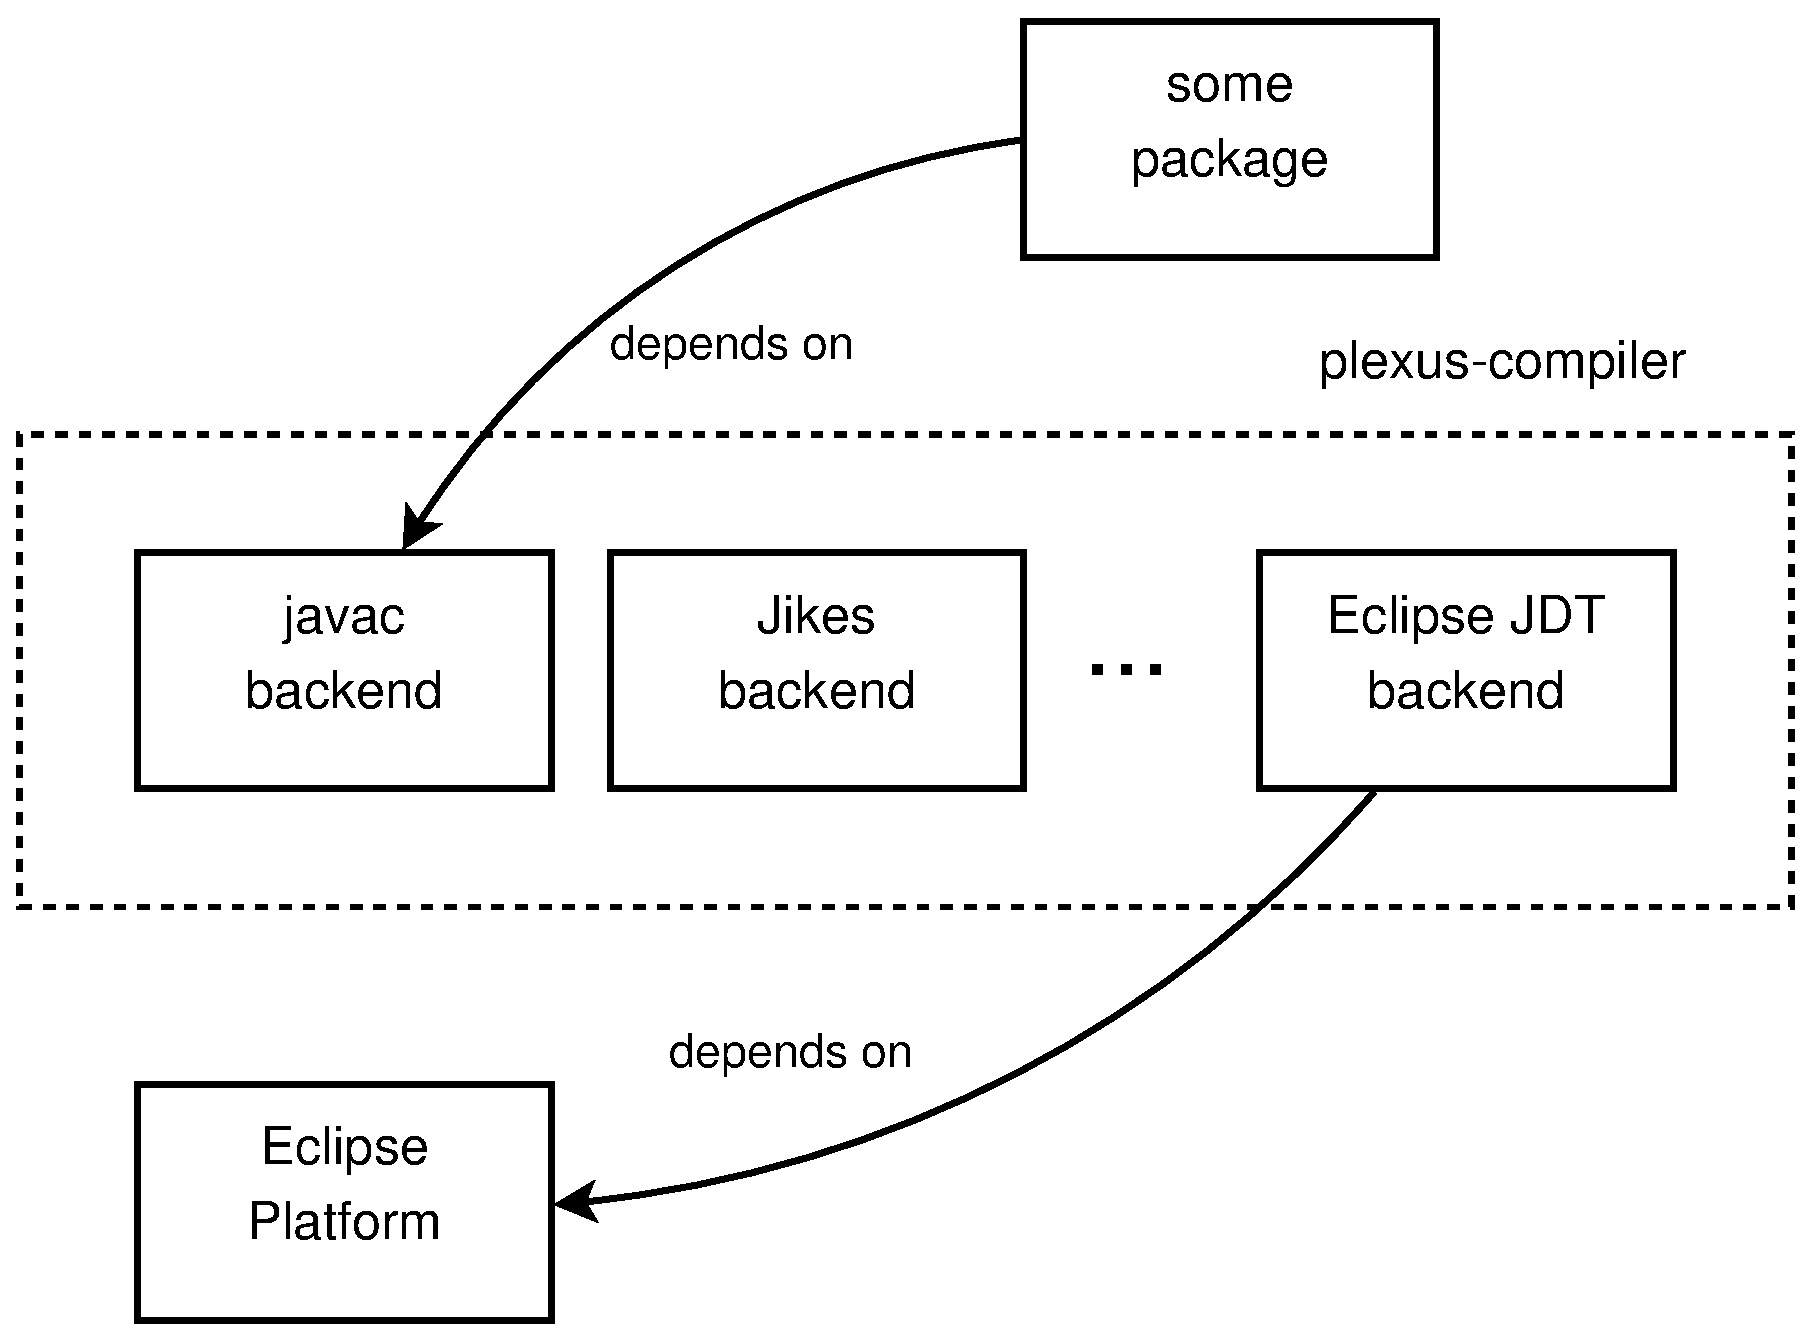
\includegraphics[scale=0.3]{plexus-compiler.eps}
  \end{center}
  \note{Maintenance of multiple subpackages is burdensome so it's not done
  usually. This causes issues when one of the artifacts pulls in big dependency
  tree. This is a recurring problem we need to solve. One of more recent
  examples was Freemind which pulled in big part of eclipse-platform in Fedora.}
\end{frame}

\section{New Maven Packaging Approach}
\begin{frame}
  \frametitle{A tool is needed}
  \begin{itemize}
    \item Simple usage
    \item Powerfull
    \item Convention over configuration
  \end{itemize}
  \note{As shown in previous exmaples, currect situation of packaging
  of Maven artifacts in Fedora requires a new tool. A tool that would
  be simple to use, doing most of the tasks for users. It should be
  powerfull enough to allow migration of all possible spec files to
  the new style of packaging, not only some of them. It should also
  utilize the convention over configuration rule so that most simple
  packages have the simpliest specx files possible, but more
  complicated cases can be handled with customizations.}
\end{frame}

\begin{frame}
  \frametitle{Structure of XMvn}
  \begin{itemize}
    \item Portable part
    \begin{itemize}
      \item pure Java
      \item integration with Maven
      \item highly configurable
      \item uses unmodified Maven
    \end{itemize}
    \item Distribution-specific part
    \begin{itemize}
      \item macros and shell scripts
      \item integration with package manager
      \item follows distribution standards
      \item automatic dependency generation
    \end{itemize}
  \end{itemize}

  \note{XMvn consists of two parts, portable part and
  distribution-specific part.

The first one is written in pure Java. It is a set of extensions to
(otherwise unmodified) Apache Maven and is licensed in consistent way
with Maven (the license is Apache License version 2.0). The portable
part has many configuration options and it tries not to rely on any
distribution-specific characteristics, so it should be possible to use
it on any GNU/Linux or Unix distribution.

The distribution-specific part forms an interface between the way how
packages are built in distributions and the portable part. For this
part is implemented only for Fedora, but different layers could be
created for different distributions, also those not based on
RPM. Among other things this part is responsible for keeping
distribution-specific defaults and automatic dependencies are
generated.}

\end{frame}


\begin{frame}[fragile]
  \frametitle{Preparation for the build}
  \begin{block}{Patching POM files}
    \scriptsize
\begin{verbatim}
%pom_add_dep org.apache.commons:commons-io
%pom_disable_module submod-foo
\end{verbatim}
  \end{block}
  \begin{block}{Launching build}
    \scriptsize
\begin{verbatim}
%mvn_file : %{name}
%mvn_build
\end{verbatim}
  \end{block}
  \note{Before the actual build is started POM files are patched using
  new Macros if needed, but usually that step is not required. Next
  the build process is configured using simple macros and the portable
  part of XMvn is launched.}
\end{frame}


\begin{frame}
  \frametitle{During build}
  \begin{itemize}
    \item Create build plan
    \item Read package metadata
    \item Call Maven to build the package
    \begin{itemize}
      \item compile sources
      \item run tests
      \item generate javadocs
    \end{itemize}
    \item Generate metadata
  \end{itemize}
  \note{During the build the configuration is read and the build plan
  is created. XML metadatata of all Maven packages installed in the
  file system is read and Maven is invoked to perform the build. After
  Maven completes the build metadata of currently built packages is
  generated.}
\end{frame}


\begin{frame}[fragile]
  \frametitle{After the build}
  \begin{block}{Installation}
    \scriptsize
\begin{verbatim}
%mvn_install
\end{verbatim}
  \end{block}
  \begin{block}{Enumerating files}
    \scriptsize
\begin{verbatim}
%files -f .mfiles
%files javadoc -f .mfiles-javadoc
\end{verbatim}
  \note{After build is finished all relevant files are installed into
  the build root and lists of installed files are created. These lists
  are then used to let RPM know which file belongs to which package.}
  \end{block}
\end{frame}


\begin{frame}[fragile]
  \begin{block}{Example spec file (part 1)}
    \scriptsize
\begin{verbatim}
Name:           maven-shared-incremental
Version:        1.0
Release:        1%{?dist}
Summary:        Maven Incremental Build support utilities
License:        ASL 2.0
URL:            http://maven.apache.org/shared/maven-shared-incremental/
Source0:        http://repo1.maven.org/maven2/org/apache/maven/[...]
BuildArch:      noarch

BuildRequires:  maven-local
BuildRequires:  plexus-component-annotations
BuildRequires:  plexus-component-api

%description
Various utility classes and plexus components for supporting
incremental build functionality in maven plugins.

%package javadoc
Summary:        API documentation for %{name}

%description javadoc
This package provides %{summary}.
\end{verbatim}
  \end{block}
  \note{A typical RPM spec file for package built using XMvn consists
  of standard package metadata (name, version, etc.), there are not
  even requires, only build requires.}
\end{frame}


\begin{frame}[fragile]
  \begin{block}{Example spec file (part 2)}
    \scriptsize
\begin{verbatim}
%prep
%setup -q

%build
%mvn_build

%install
%mvn_install

%files -f .mfiles
%doc LICENSE NOTICE
%dir %{_javadir}/%{name}

%files javadoc -f .mfiles-javadoc
%doc LICENSE NOTICE

%changelog
* Wed Jan 23 2013 Mikolaj Izdebski <mizdebsk@redhat.com> - 1.0-1
- Initial packaging



\end{verbatim}
  \end{block}
  \note{Build and install sections are usually very simple, possiblt
  single-line. In files sections only non-maven files (like license
  texts or documentation files) need to be listed, everything
  Macen-specific is handled automatucally.}
\end{frame}

\begin{frame}
  \frametitle{Advantages}
  \begin{itemize}
    \item Simpler, more readable packages
    \item Easier and faster packaging and updates
    \item Better quality packages
    \item Reduced metadata redundancy
    \item No modifications to Maven
    \item Changes in guidelines are easier to introduce
  \end{itemize}
  \note{From previous examples its clear that the new way of packaging
  Maven artifacts has numerous advantages.}
\end{frame}

\begin{frame}[fragile]
  \frametitle{Easier Maven maintenance}
  \begin{block}{Maven diff}
    \scriptsize
\begin{verbatim}
 0001-Add-plugin-api-deps.patch                |  28 --
 0001-Customize-compiler-plugin.patch          | 104 ------
 0002-Use-custom-resolver.patch                | 224 -------------
 0003-Use-utf-8-source-encoding.patch          |  24 --
 ...-scope-skipping-with-maven.test.skip.patch | 160 ---------
 ...ompiler-plugin-default-to-source-1.5.patch |  33 --
 JavadirWorkspaceReader.java                   | 198 -----------
 MavenJPackageDepmap.java                      | 313 ------------------
 maven-empty-dep.jar                           | Bin 341 -> 0 bytes
 maven-empty-dep.pom                           |   9 -
 maven-script-local                            |  47 ---
 maven-script-rpmbuild                         |  93 ------
 maven.spec                                    | 269 +++------------
 repo-metadata.tar.xz                          | Bin 3028 -> 0 bytes
 14 files changed, 37 insertions(+), 1465 deletions(-)
\end{verbatim}
  \note{All Fedora-specific Maven customizations could be removed,
  which means much easier Maven maintenance in Fedora.}
  \end{block}
\end{frame}


\begin{frame}[fragile]
  \frametitle{Build description of maven-surefire in F-12}
  \scriptsize
  \begin{verbatim}
%if %{with_maven}
    export MAVEN_REPO_LOCAL=$(pwd)/.m2/repository
    mkdir -p $MAVEN_REPO_LOCAL
    cat %{SOURCE4}
    mvn-jpp -e -Dmaven.repo.local=$MAVEN_REPO_LOCAL \
        -Dmaven2.jpp.depmap.file=%{SOURCE4} \
        -Dmaven.test.skip=true install
    for dir in maven-surefire-plugin maven-surefire-report-plugin \
               surefire-api surefire-booter surefire-providers/surefire-junit; do
        (cd $dir
         mvn-jpp -Dmaven.repo.local=$MAVEN_REPO_LOCAL \
                 -Dmaven2.jpp.depmap.file=%{SOURCE4} \
                 javadoc:javadoc
        )
    done
%else
    mkdir -p lib
    build-jar-repository -s -p lib classworlds junit plexus/utils
    ant -Dmaven.mode.offline=true
    cp -p target/*jar ../lib/$project.jar
%endif
  \end{verbatim}
  \note{That's how the build section of an example spec file used to
  look like in Fedora 12.}
\end{frame}

\begin{frame}[fragile]
  \frametitle{Build description of maven-surefire in F-15}
  \scriptsize
  \begin{verbatim}
# tests turned off because they need jmock
mvn-rpmbuild -e \
        -Dmaven.local.depmap.file=%{SOURCE1} \
        -Dmaven.test.skip=true \
        install javadoc:aggregate
  \end{verbatim}
  \note{That's how build section of the same package used to look
  in Fedora 15.}
\end{frame}

\begin{frame}[fragile]
  \frametitle{Build description of maven-surefire in F-19}
  \scriptsize
  \begin{verbatim}
%mvn_build -f
  \end{verbatim}
  \note{And that's Fedora 19. This example speaks for itself.}
\end{frame}


\begin{frame}[fragile]
  \frametitle{Simplified package}
  \begin{block}{maven-surefire diff between F-12 and F-18}
    \scriptsize
\begin{verbatim}
 .cvsignore                           |   3 -
 .gitignore                           |  14 +
 Makefile                             |  21 --
 maven-surefire-2.3-junit4-pom.patch  |  11 -
 maven-surefire-booter-build.xml      |  64 -----
 maven-surefire-build.xml             |  90 ------
 maven-surefire-buildonlyjunit3.patch |  13 -
 maven-surefire-buildskiptestng.patch |  12 -
 maven-surefire-jpp-depmap.xml        |  23 --
 maven-surefire-plexus12.patch        |  20 --
 maven-surefire.spec                  | 399 +++++++--------------------
 sources                              |   3 +-
 12 files changed, 117 insertions(+), 556 deletions(-)
\end{verbatim}
  \end{block}
  \note{Packaging of multi-artifact packages was simplified
  considerably. This can be seen in an example difference between
  Fedora 12 and Fedora 19 package.}
\end{frame}

\begin{frame}
  \frametitle{Disadvantages}
  \begin{itemize}
    \item Harder to debug
    \item Incompatibility with older systems
    \item Bleeding edge
  \end{itemize}
  \note{XMvn as any solution solution has its disadvantages too,
  but it's believed that all the advantages surpass them.}
\end{frame}

\begin{frame}
  \frametitle{Summary}
  \begin{itemize}
    \item Improved packaging
    \item Full solution
    \item Backwards-compatible
    \item Smooth transition
  \end{itemize}
\end{frame}


\begin{frame}
  \frametitle{Future}
  \begin{itemize}
    \item Automated package generation
    \item Debugging tools
    \item Graphical tooling
    \item Support for more types of artifacts
    \item Integration with Eclipse
    \item Adoption by different distributions?
  \end{itemize}
  \note{Any software that is useful has to be changed,
  so hopefully XMvn future will bring many changes.}
\end{frame}


\begin{frame}
  \frametitle{Links}
  \begin{itemize}
    \item Code repository
    \begin{itemize}
    \item \url{http://git.fedorahosted.org/git/xmvn.git}
      \end{itemize}
    \item Fedora 19 feature
    \begin{itemize}
      \item \url{http://fedoraproject.org/wiki/Features/XMvn}
    \end{itemize}
    \item Cookbook
    \begin{itemize}
      \item \url{http://mizdebsk.fedorapeople.org/xmvn/cookbook/}
    \end{itemize}
  \end{itemize}
\end{frame}



\mode<presentation> {
  \Rhbg{\frame{\theend}}
}

\end{document}
